
\documentclass[12pt]{article}
\usepackage[utf8]{inputenc}
\usepackage{graphicx}
\usepackage{amsmath}
\usepackage{booktabs}
\usepackage{caption}
\usepackage{subcaption}
\usepackage{geometry}
\usepackage{hyperref}
\usepackage{float}
\usepackage{enumitem}
\usepackage{xcolor}

% Page geometry
\geometry{a4paper, margin=1in}

% Hyperref settings
\hypersetup{
    colorlinks=true,
    linkcolor=blue,
    filecolor=magenta,
    urlcolor=cyan
}

% Custom commands
\newcommand{\datasetname}[1]{\textbf{#1}}
\newcommand{\paramname}[1]{\texttt{#1}}

% Title page
\begin{document}
\begin{titlepage}
    \centering
    \vspace*{2cm}

    % Logo
    
\includegraphics[width=0.4\textwidth]{scagentic_logo.png}
    \vspace{1cm}

    % Title
    \Huge\textbf{Single-Cell RNA-seq Analysis Report}
    \vspace{1cm}

    % Study information
    \Large\textbf{sample 8510, patient 1 post-treatment biopsy, scRNA-seq}
    \vspace{0.5cm}

    % GEO accession
    \Large\textbf{GEO Accession: GSM7770557}
    \vspace{0.5cm}

    % Species and tissue
    \Large\textbf{Species: Homo sapiens}
    \vspace{0.5cm}
    \vspace{1cm}

    % Date
    \large\today
\end{titlepage}

% Table of contents
\tableofcontents
\newpage

% Study information
\section{Study Information}
\begin{itemize}
    \item \textbf{GEO Accession:} GSM7770557
    \item \textbf{Status:} Public on Sep 12, 2023
    \item \textbf{Title:} sample 8510, patient 1 post-treatment biopsy, scRNA-seq
    \item \textbf{Source Name:} brain
    \item \textbf{Organism:} Homo sapiens
    \item \textbf{Analysis Date:} {April 05, 2025}
\end{itemize}

% Add a link to the GEO page
\begin{quote}
    \textbf{GEO Link:} \url{https://www.ncbi.nlm.nih.gov/geo/query/acc.cgi?acc=GSM7770557}
\end{quote}

% Analysis parameters
\section{Analysis Parameters}
\begin{table}[H]
    \centering
    \begin{tabular}{ll}
        \toprule
        \textbf{Parameter} & \textbf{Value} \\
        \midrule
        Min Genes & 200 \\
        Min Cells & 3 \\
        Max Percent Mt & 20 \\
        N Top Genes & 2000 \\
        N Pcs & 50 \\
        Resolution & 0.5 \\

        \bottomrule
    \end{tabular}
    \caption{Analysis parameters used in preprocessing}
    \label{tab:parameters}
\end{table}

% Analysis Pipeline
\section{{Analysis Pipeline}}

\subsection{1. Quality Control}
Calculated quality control metrics and generated distribution plots for genes, counts, and mitochondrial content. The violin plots show: (1) The number of genes expressed in the count matrix, (2) The total counts per cell, and (3) The percentage of counts in mitochondrial genes. It is useful to consider QC metrics jointly by inspecting a scatter plot colored by pct\_counts\_mt.

\begin{figure}[H]
    \centering
    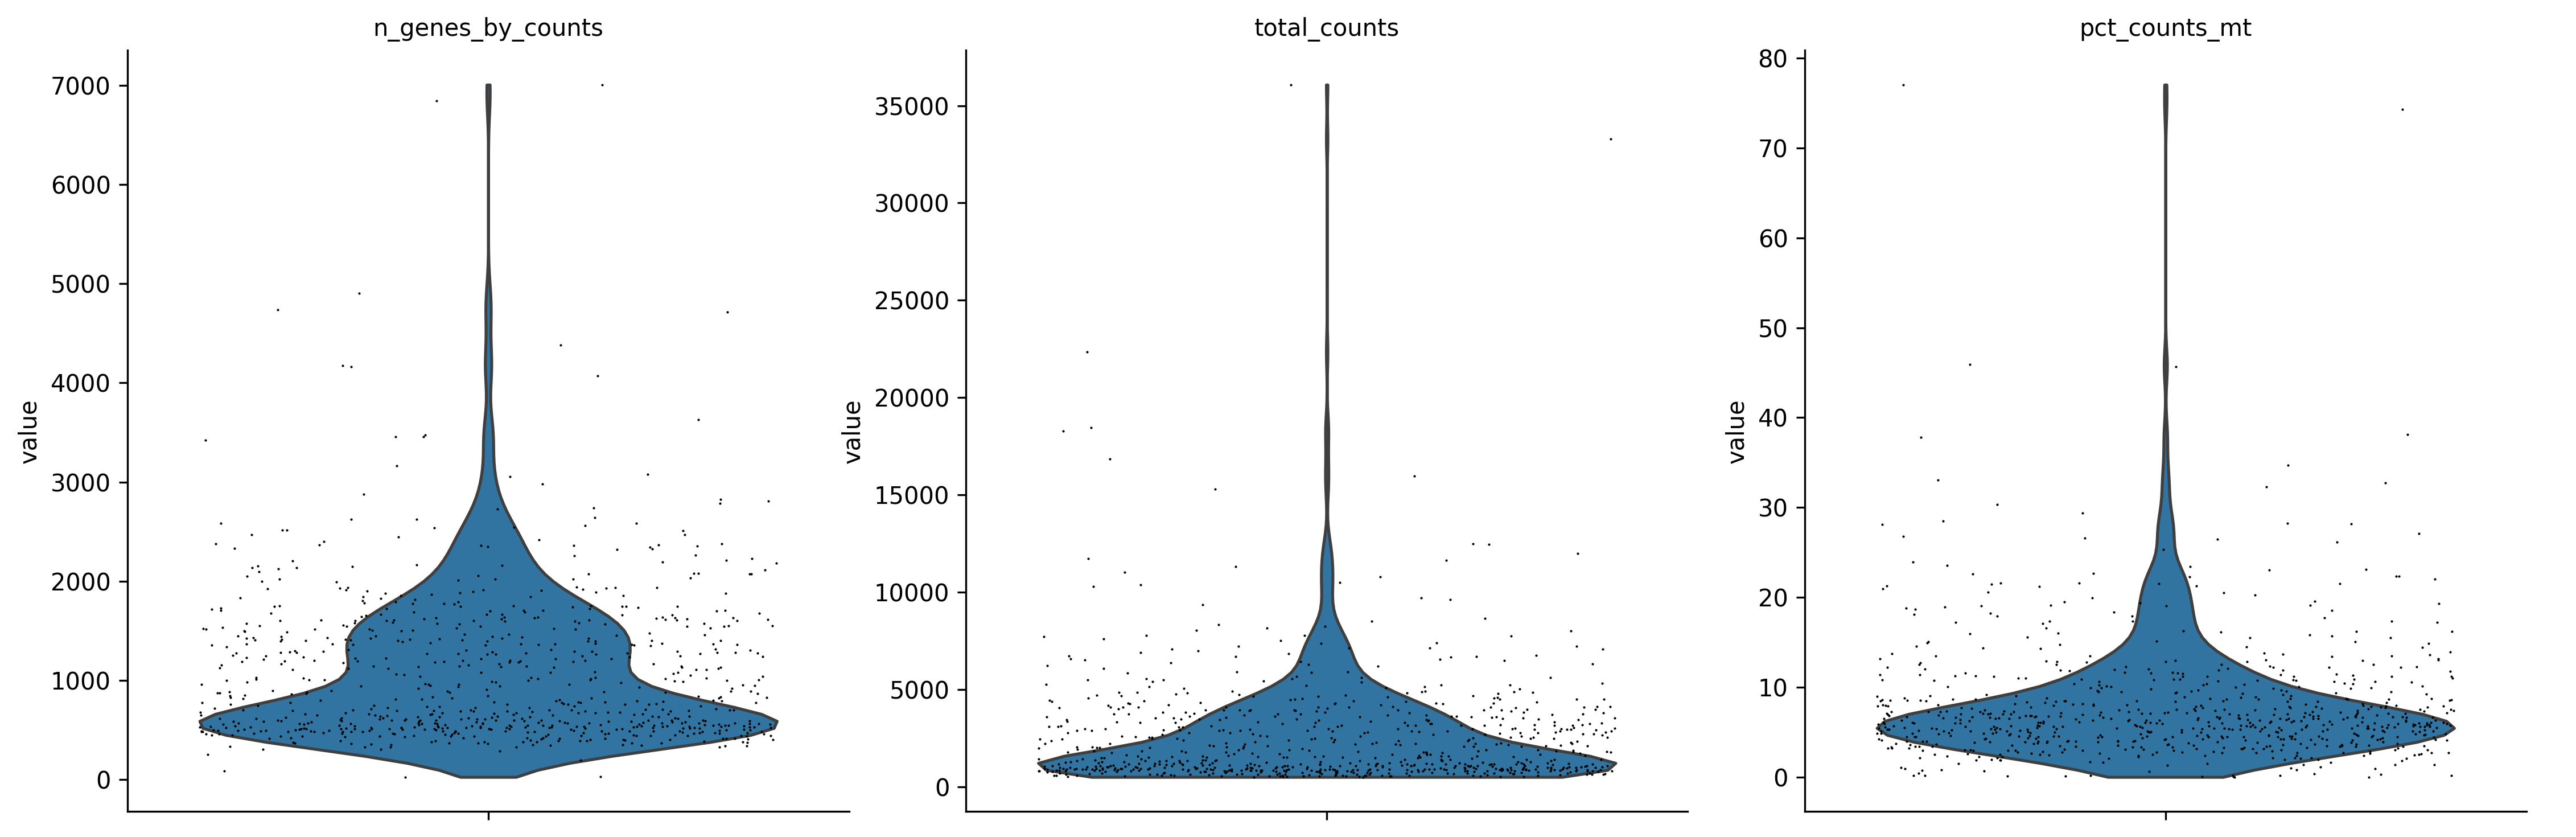
\includegraphics[width=0.8\textwidth]{qc_distributions.png}
    \caption{Quality Control}
    \label{fig:qc_distributions}
\end{figure}

\begin{figure}[H]
    \centering
    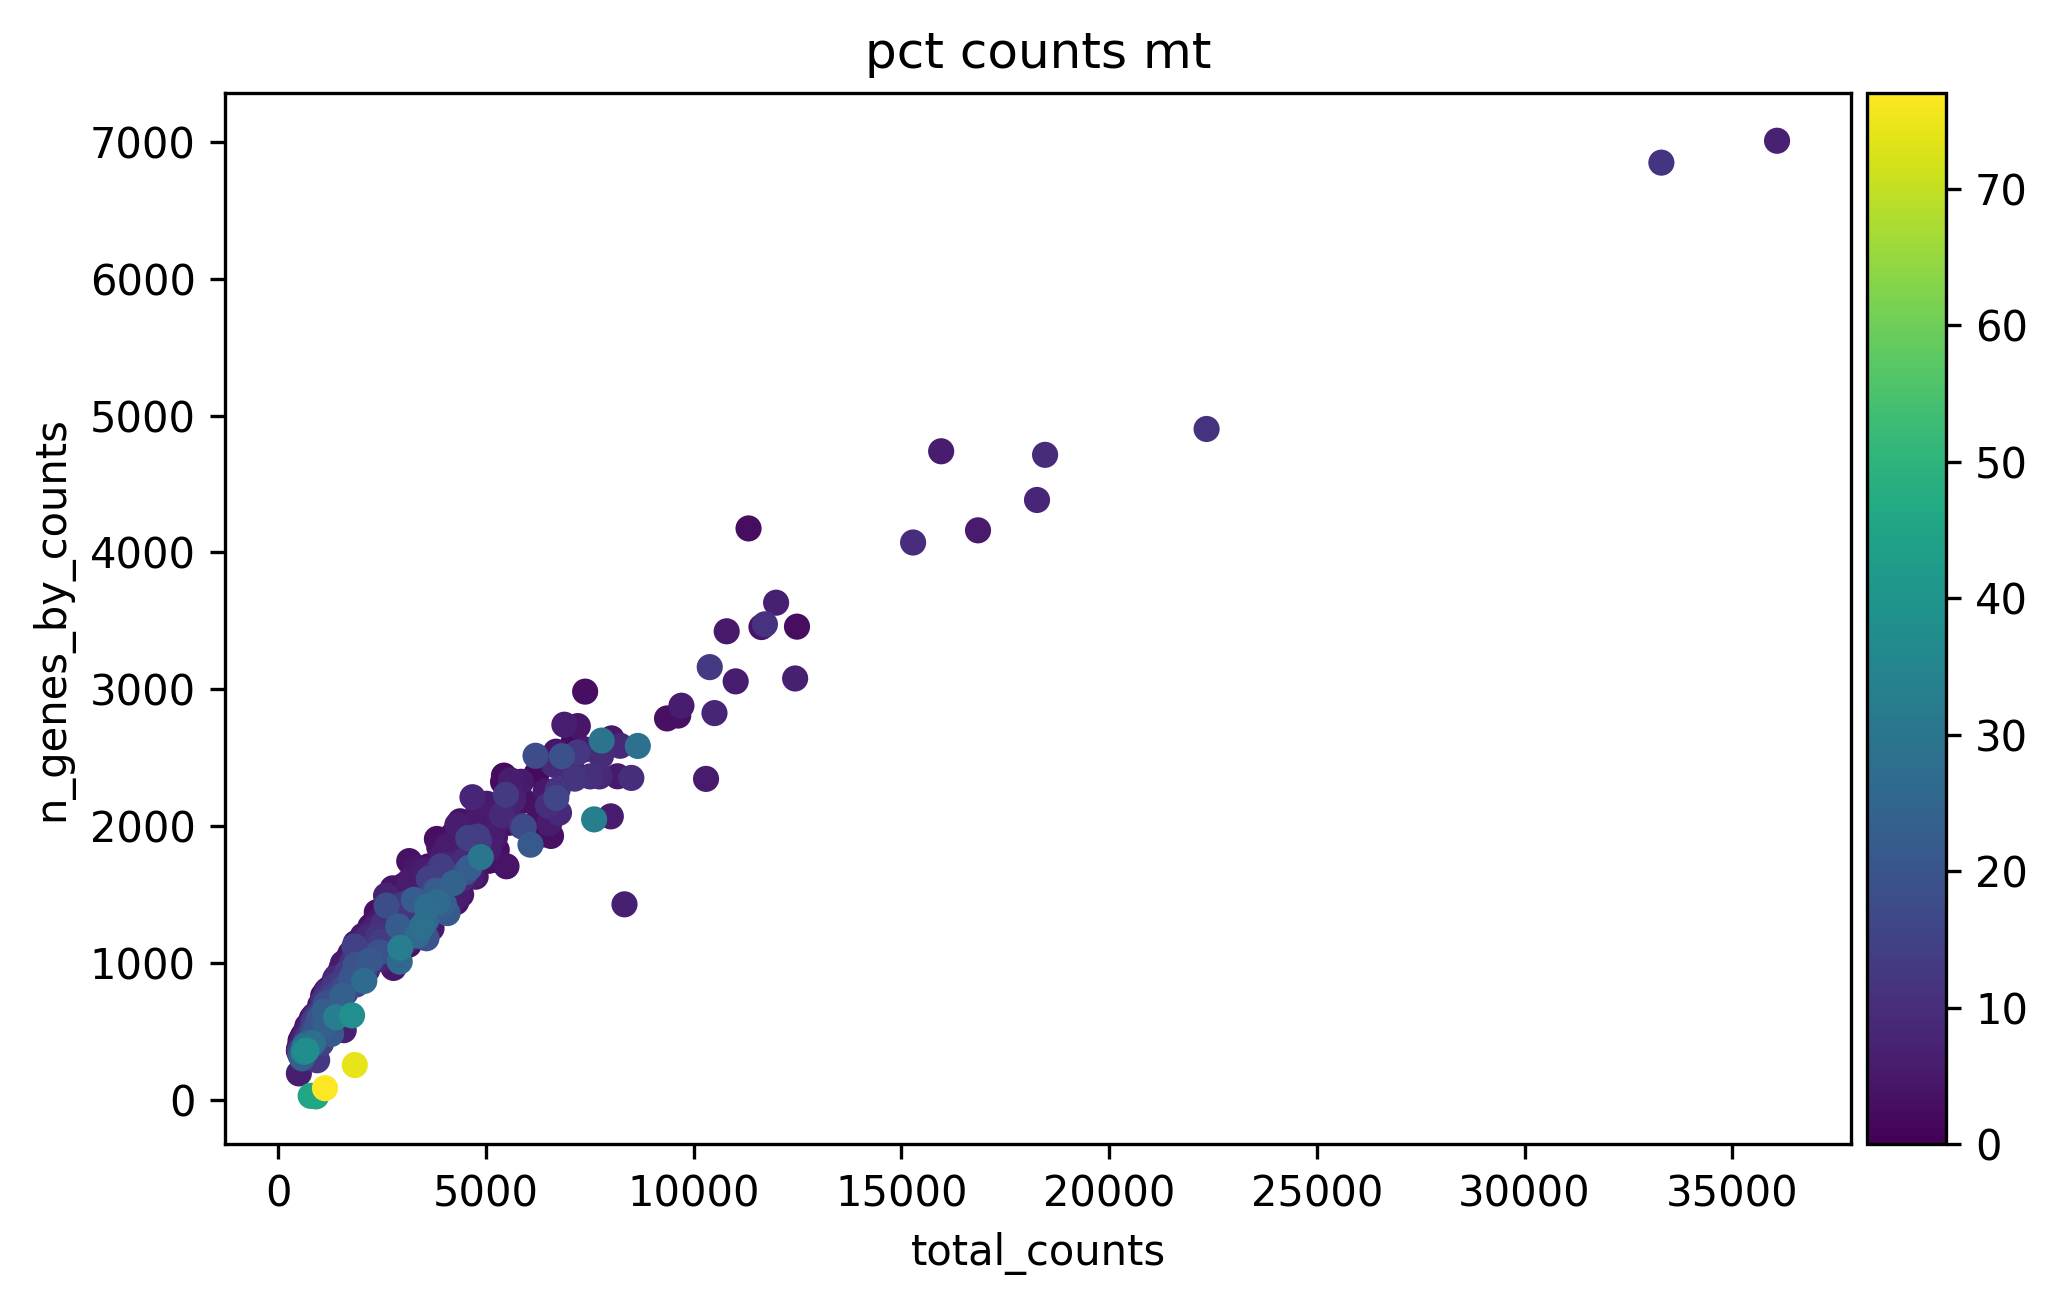
\includegraphics[width=0.8\textwidth]{qc_scatter.png}
    \caption{Additional QC visualization: Scatter plot of total counts vs. number of genes, colored by mitochondrial content percentage}
    \label{fig:qc_scatter}
\end{figure}

\subsection{2. Filtering Cells}
Based on the QC metric plots, one could now remove cells that have too many mitochondrial genes expressed or too many total counts by setting manual or automatic thresholds. However, sometimes what appears to be poor QC metrics can be driven by real biology so we suggest starting with a very permissive filtering strategy and revisiting it at a later point. We therefore now only filter cells and genes based on the Quality Control plots and report these filtered cells and genes in this section. Additionally, it is important to note that for datasets with multiple batches, quality control should be performed for each sample individually as quality control thresholds can vary substantially between batches.

Filtered cells with at least 200 genes, genes expressed in at least 3 cells, and cells with less than 20\% mitochondrial content.

\subsection{3. Doublet Detection}
As a next step, we run a doublet detection algorithm. Identifying doublets is crucial as they can lead to misclassifications or distortions in downstream analysis steps. Scanpy contains the doublet detection method Scrublet [Wolock2019]. Scrublet predicts cell doublets using a nearest-neighbor classifier of observed transcriptomes and simulated doublets. One can either filter directly on predicted\_doublet or use the doublet\_score later during clustering to filter clusters with high doublet scores. In this step, we filter directly on predicted\_doublet. You can change it later by interacting in the chat.

\subsection{4. Normalization and Scaling}
The next preprocessing step is normalization. A common approach is count depth scaling with subsequent log plus one (log1p) transformation. Count depth scaling normalizes the data to a "size factor" such as the median count depth in the dataset, ten thousand (CP10k) or one million (CPM, counts per million). We are applying median count depth normalization with log1p transformation (AKA log1PF). The size factor for count depth scaling can be controlled via target\_sum in pp.normalize\_total. After normalization, we scaled the data to have zero mean and unit variance.

\subsection{5. Feature Selection}
As a next step, we want to reduce the dimensionality of the dataset and only include the most informative genes. This step is commonly known as feature selection. Here we use the scanpy function pp.highly\_variable\_genes that annotates highly variable genes by reproducing the implementations of Seurat [Satija2015], Cell Ranger [Zheng2017], and Seurat v3 [Stuart2019] depending on the chosen flavor. We selected the top 2000 highly variable genes for downstream analysis.

\begin{figure}[H]
    \centering
    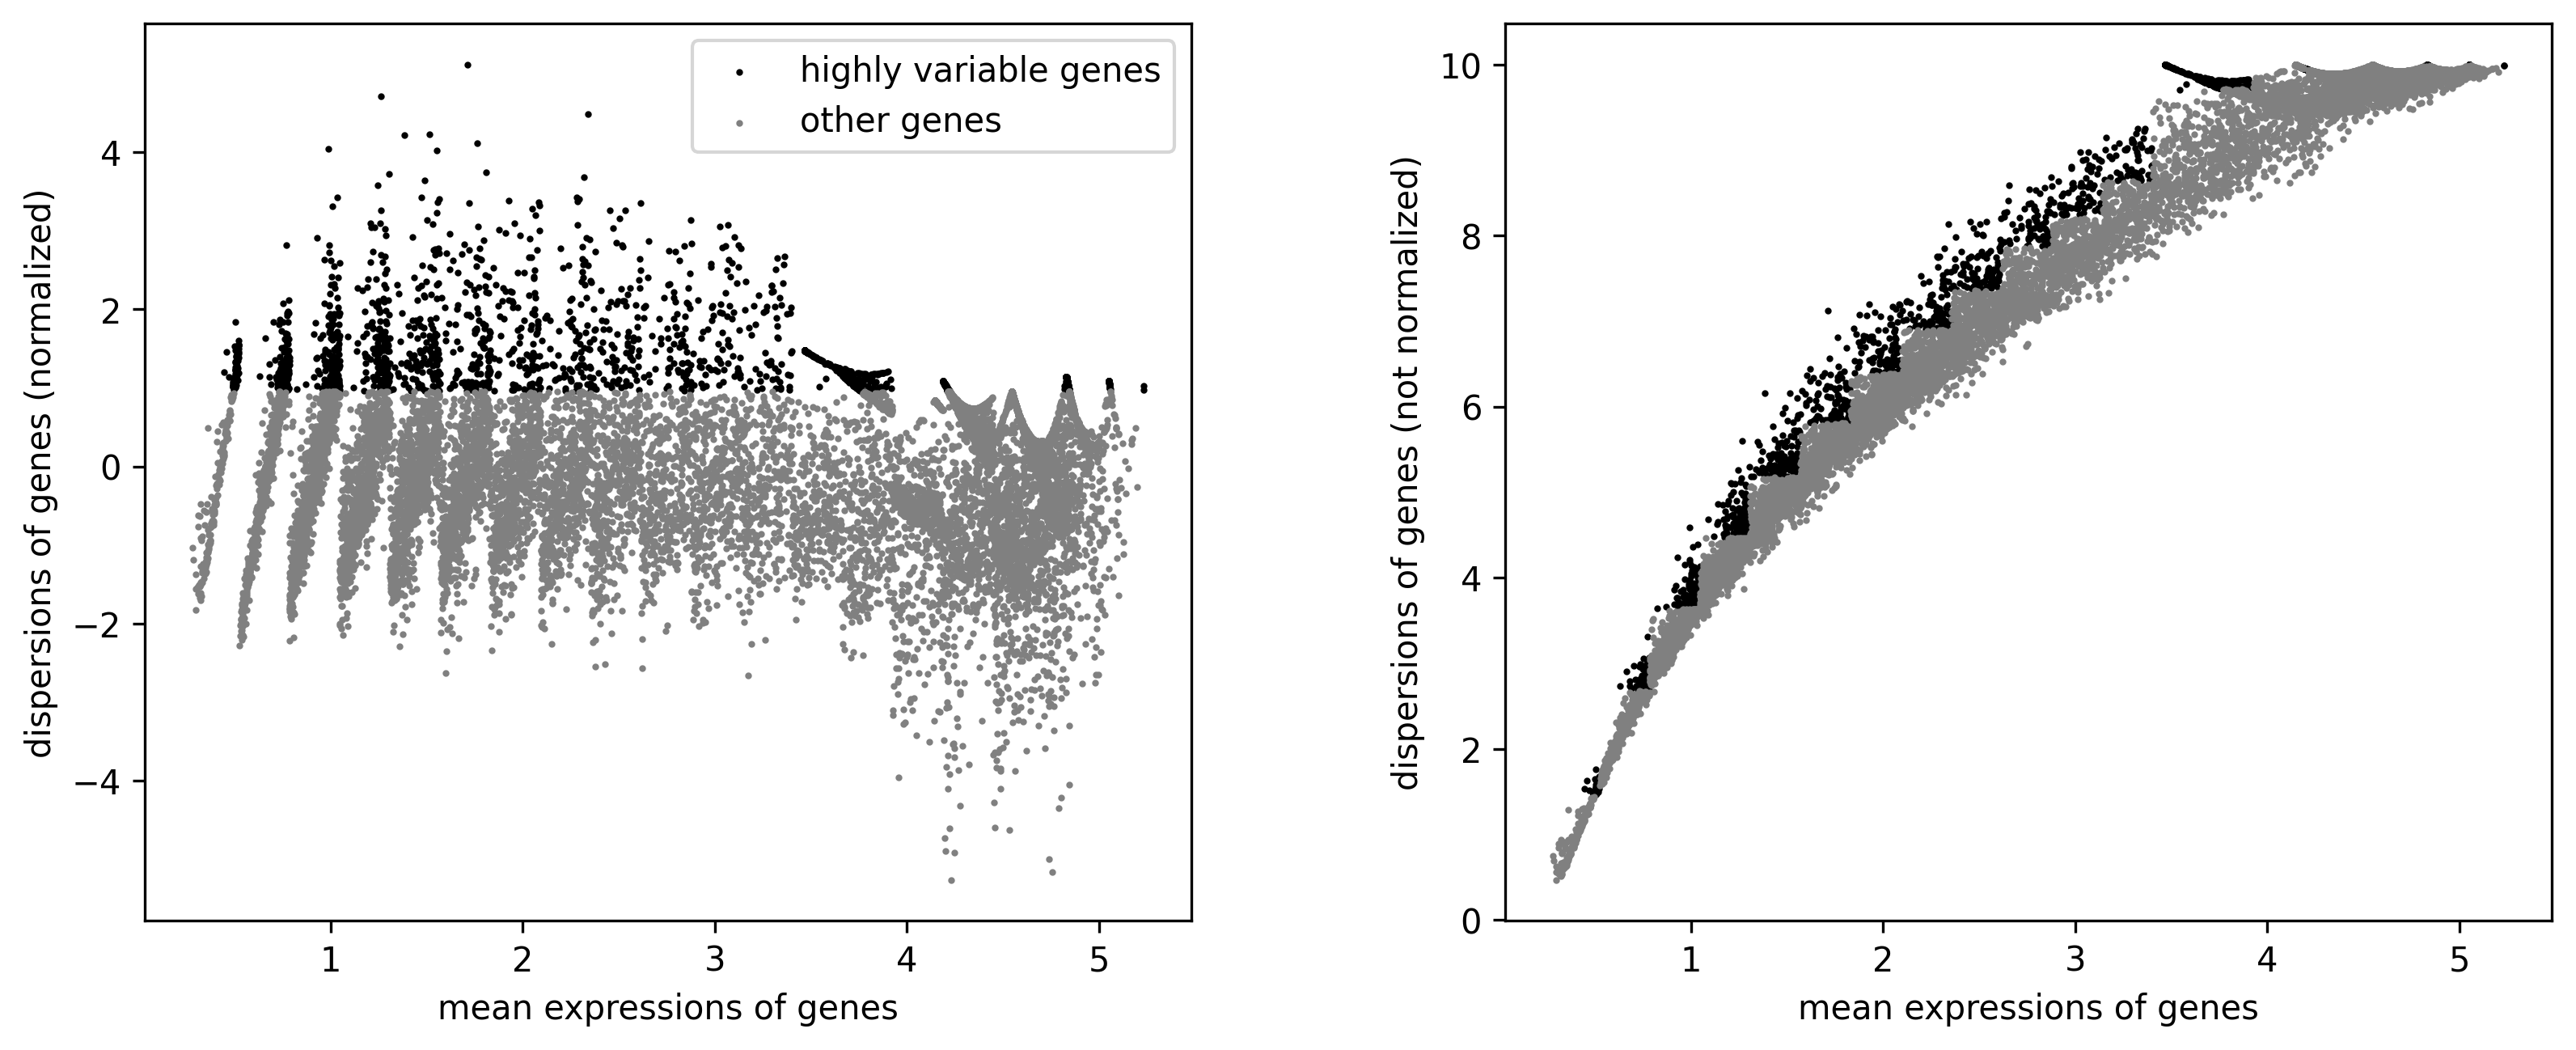
\includegraphics[width=0.8\textwidth]{highly_variable_genes.png}
    \caption{Feature Selection}
    \label{fig:highly_variable_genes}
\end{figure}

\subsection{6. Dimensionality Reduction}
Reduce the dimensionality of the data by running principal component analysis (PCA), which reveals the main axes of variation and denoises the data. We inspect the contribution of single PCs to the total variance in the data. This gives us information about how many PCs we should consider in order to compute the neighborhood relations of cells, e.g. used in the clustering function Leiden or tSNE. In experience, there does not seem to be signifigant downside to overestimating the numer of principal components. We can also plot the principal components to see if there are any potentially undesired features (e.g. QC metrics) driving signifigant variation in this dataset. In the case there isn't anything too alarming, but it's still a good idea to explore this.

\begin{figure}[H]
    \centering
    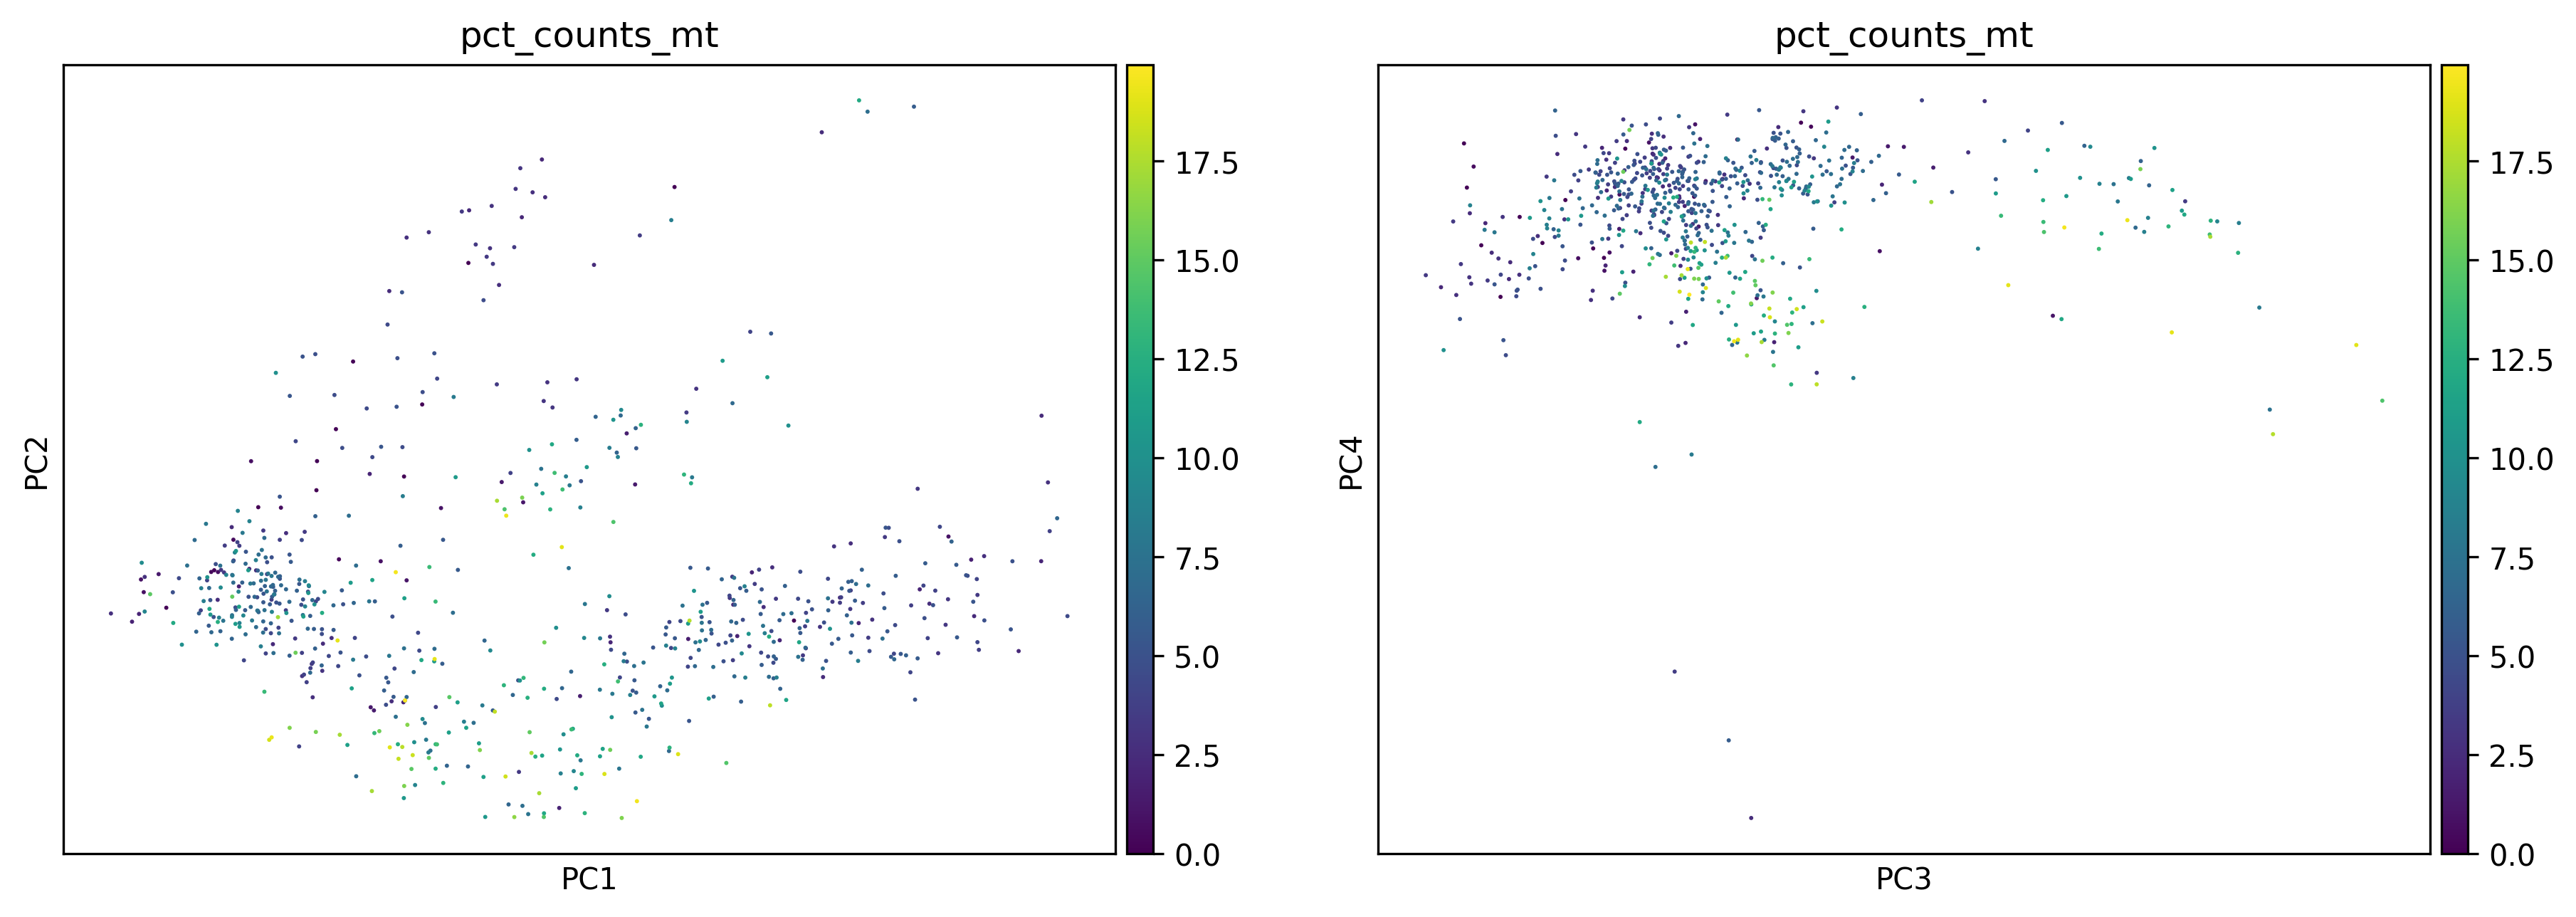
\includegraphics[width=0.8\textwidth]{pca_metrics.png}
    \caption{Dimensionality Reduction}
    \label{fig:pca_metrics}
\end{figure}

\subsection{7. Nearest Neighbor Graph Construction}
We compute the neighborhood graph of cells using the PCA representation of the data. This graph can then be embedded in two dimensions for visualization with UMAP (McInnes et al., 2018). If you inspect batch effects in your UMAP it can be beneficial to integrate across samples and perform batch correction/integration. We use scanorama and scvi-tools for batch integration.

\subsection{8. Clustering}
As with Seurat and many other frameworks, we recommend the Leiden graph-clustering method (community detection based on optimizing modularity) [Traag2019]. Note that Leiden clustering directly clusters the neighborhood graph of cells, which we already computed in the previous section.

\begin{figure}[H]
    \centering
    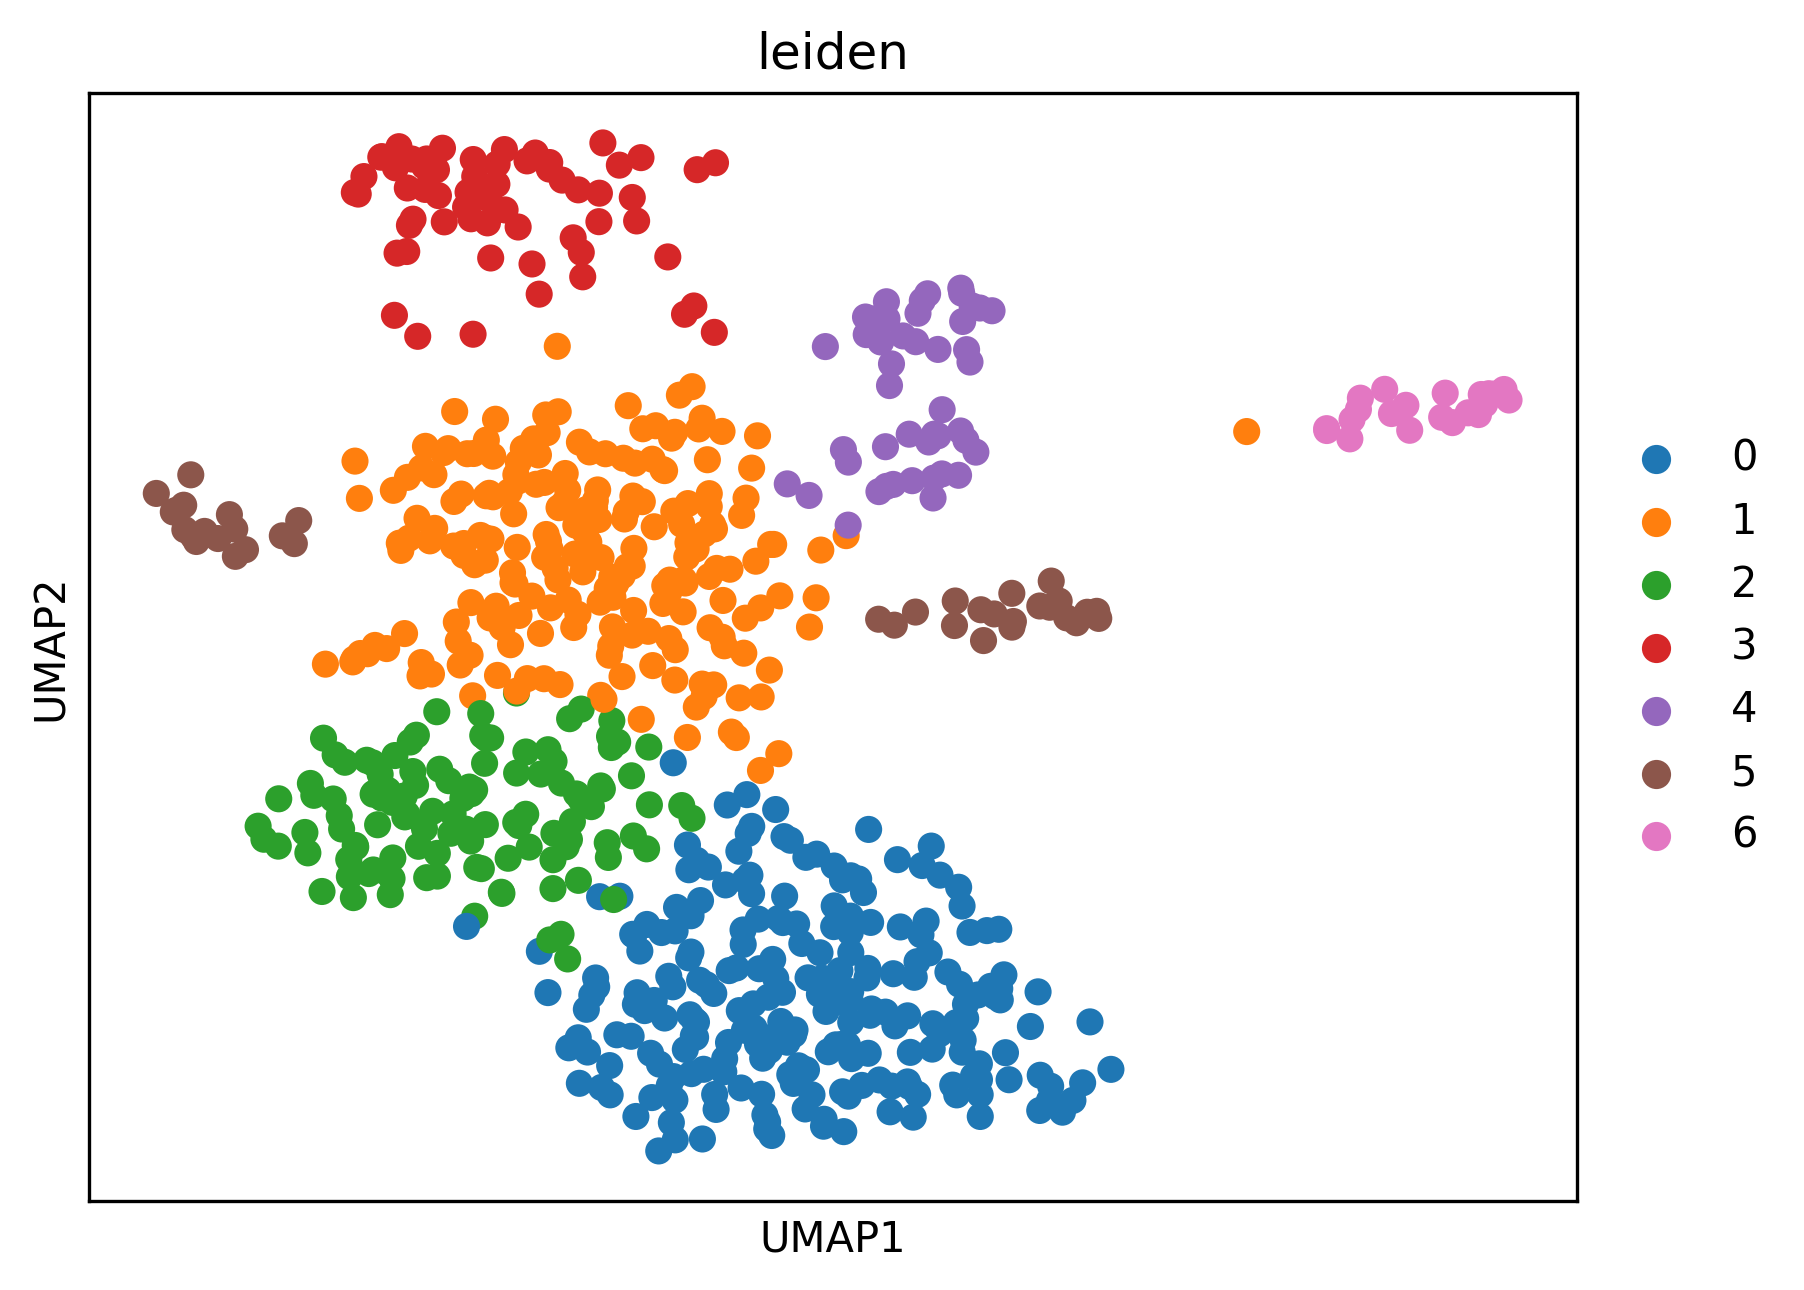
\includegraphics[width=0.8\textwidth]{umap_clusters.png}
    \caption{Clustering}
    \label{fig:umap_clusters}
\end{figure}

\subsection{9. Re-assess Quality Control and Cell Filtering}
As indicated before, we will now re-assess our filtering strategy by visualizing different QC metrics using UMAP. Additionally, we visualize the distribution of predicted doublets and doublet scores across clusters to assess the quality of our doublet detection.

\begin{figure}[H]
    \centering
    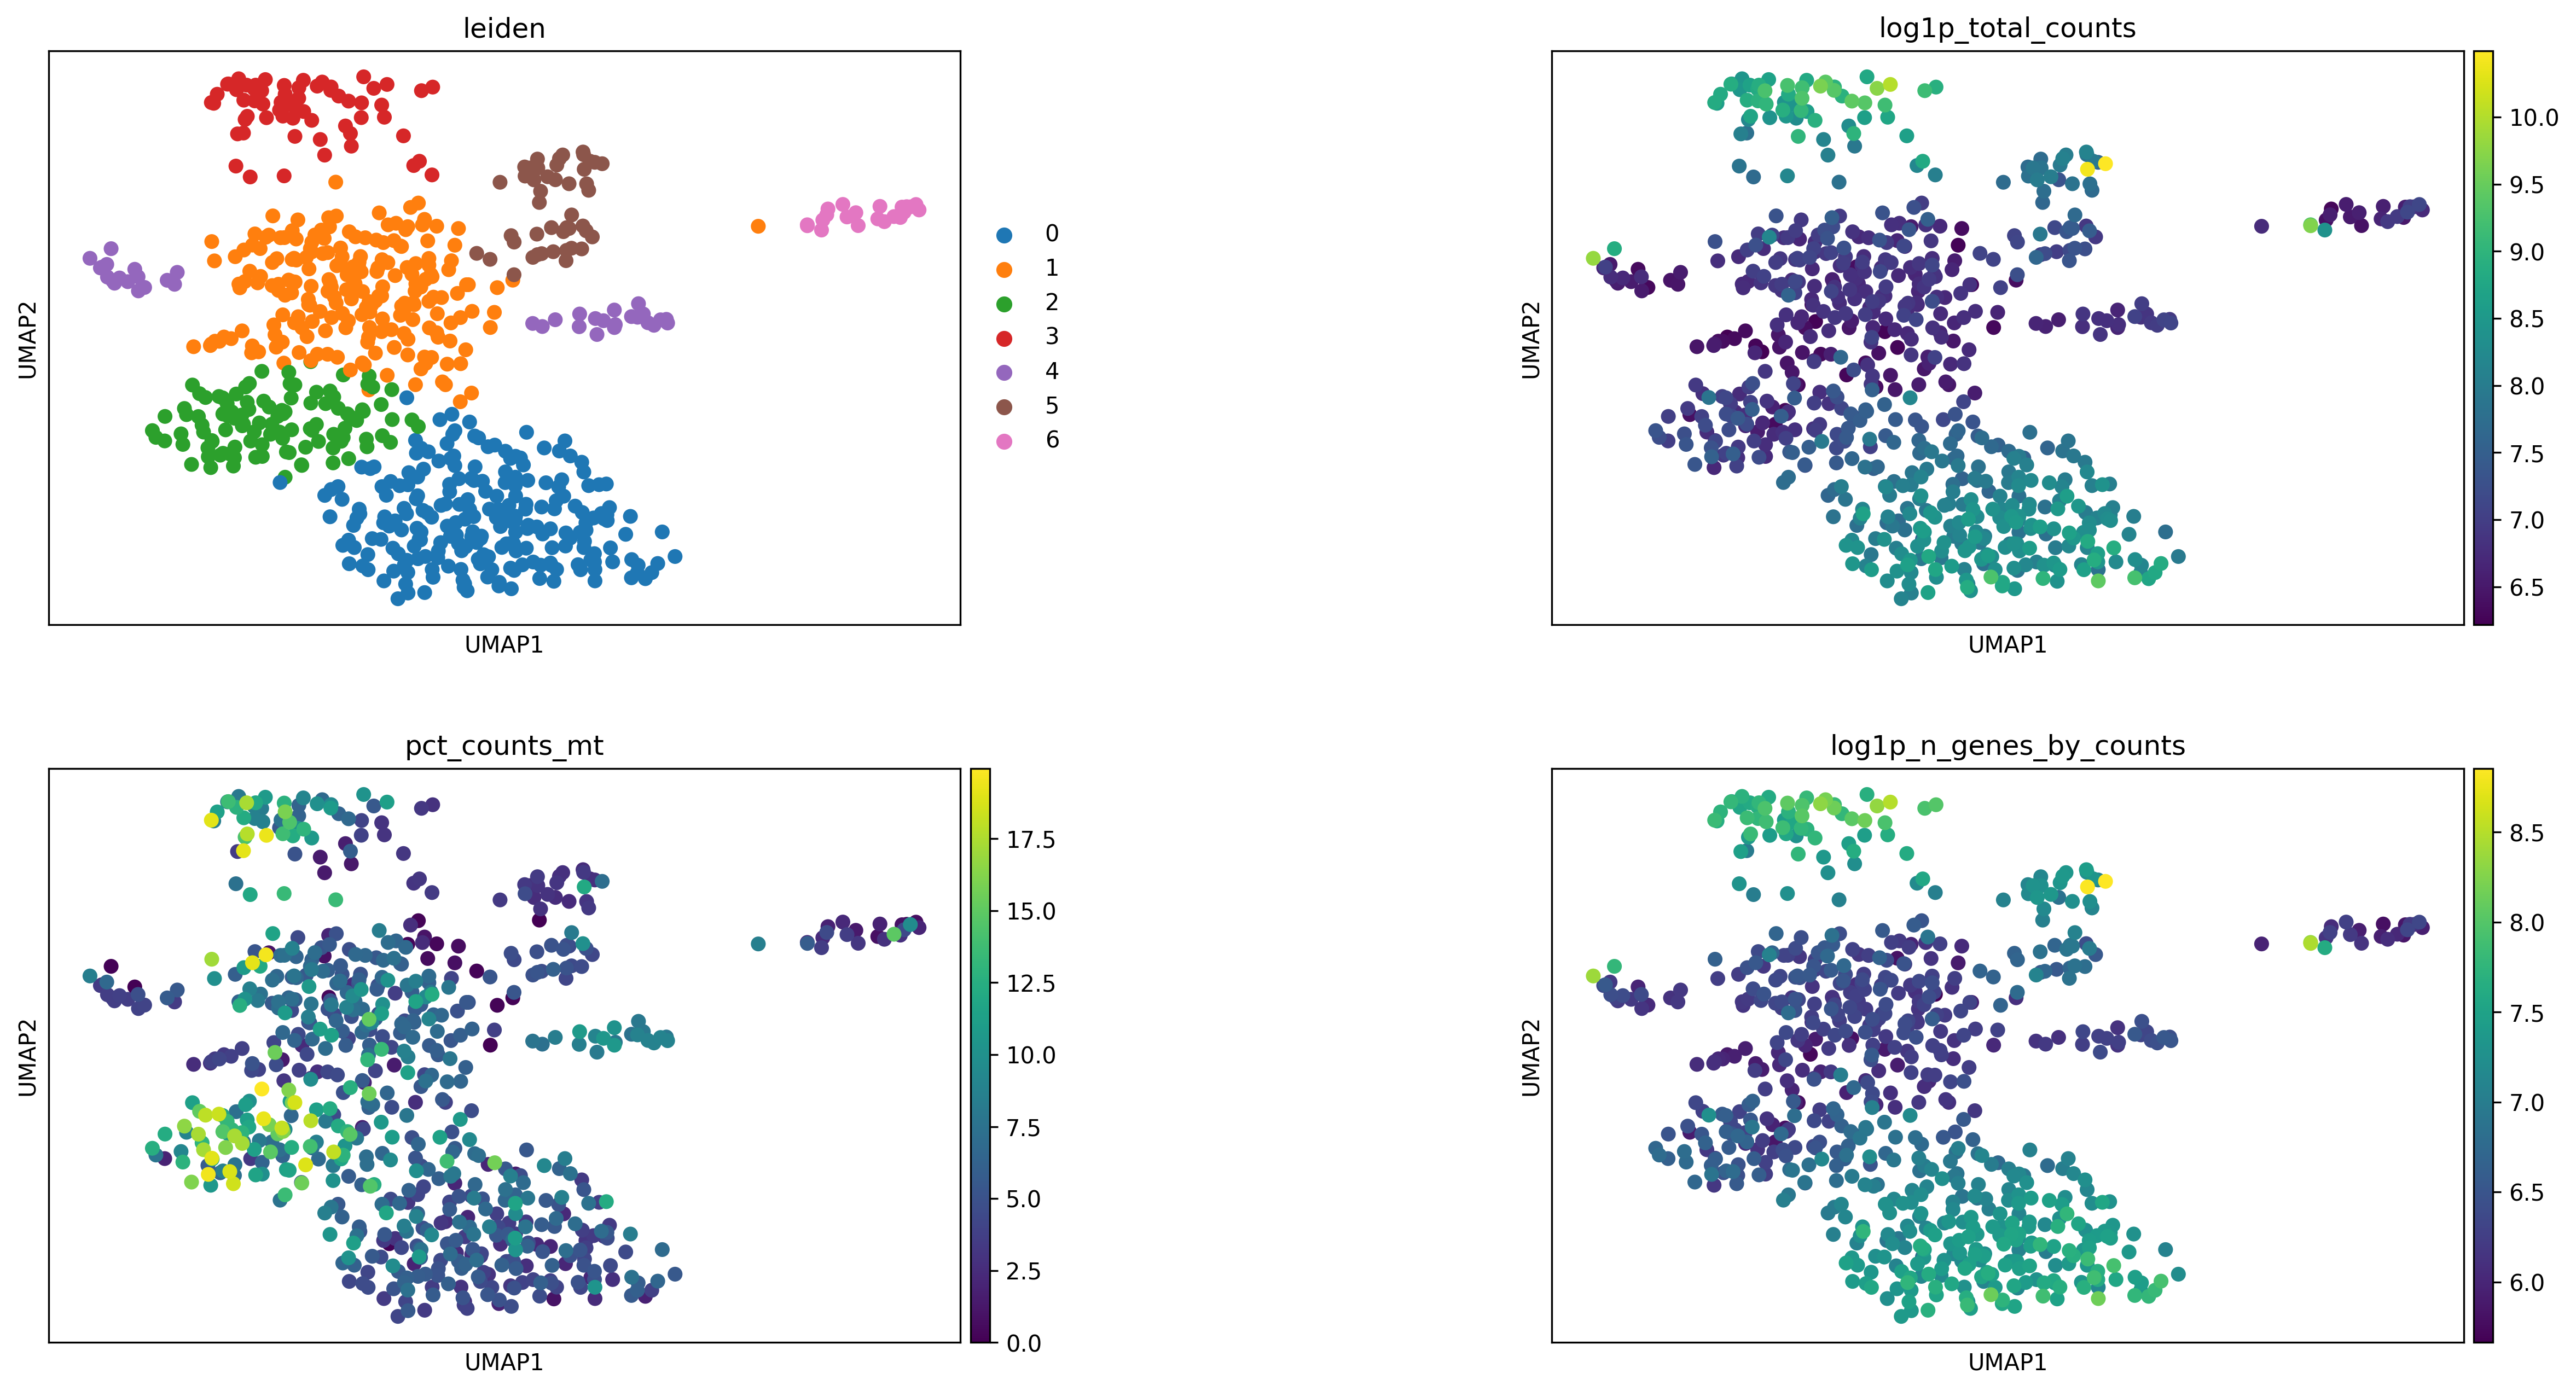
\includegraphics[width=0.8\textwidth]{umap_qc.png}
    \caption{Re-assess Quality Control and Cell Filtering}
    \label{fig:umap_qc}
\end{figure}

\begin{figure}[H]
    \centering
    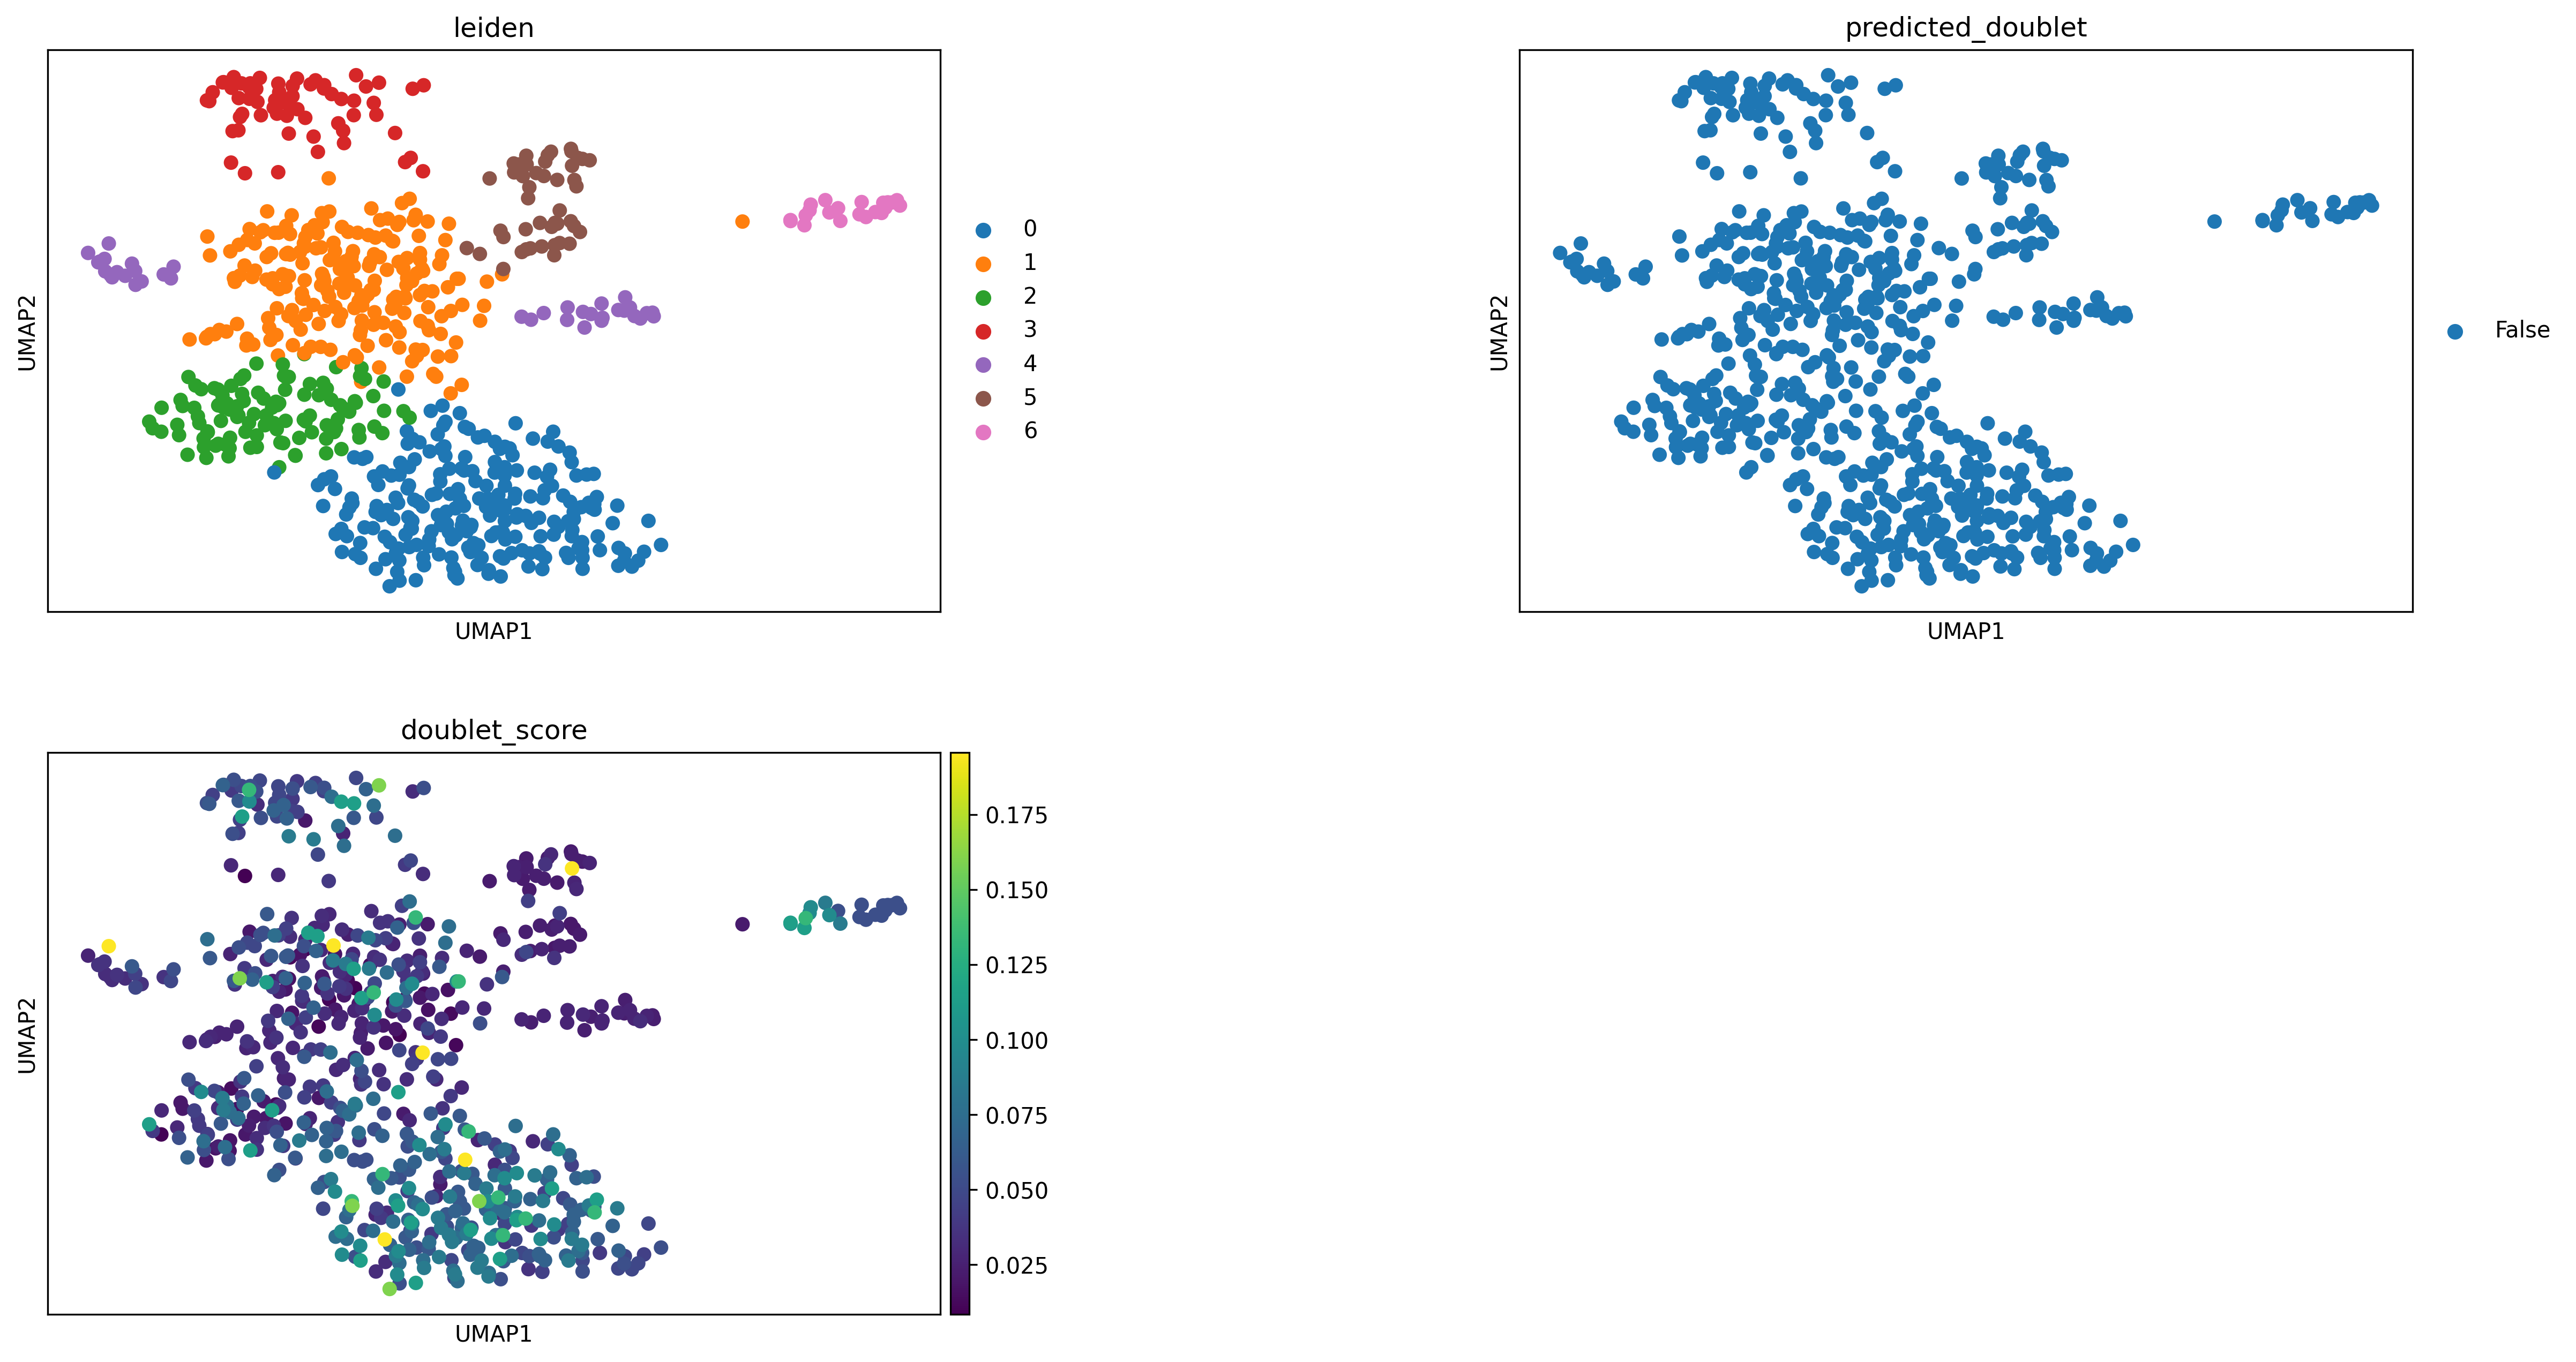
\includegraphics[width=0.8\textwidth]{umap_doublets_qc.png}
    \caption{Re-assess Quality Control and Cell Filtering}
    \label{fig:umap_doublets_qc}
\end{figure}

\subsection{10. Differential Expression Analysis}
Identified differentially expressed genes between clusters using the Wilcoxon rank-sum test.

\begin{figure}[H]
    \centering
    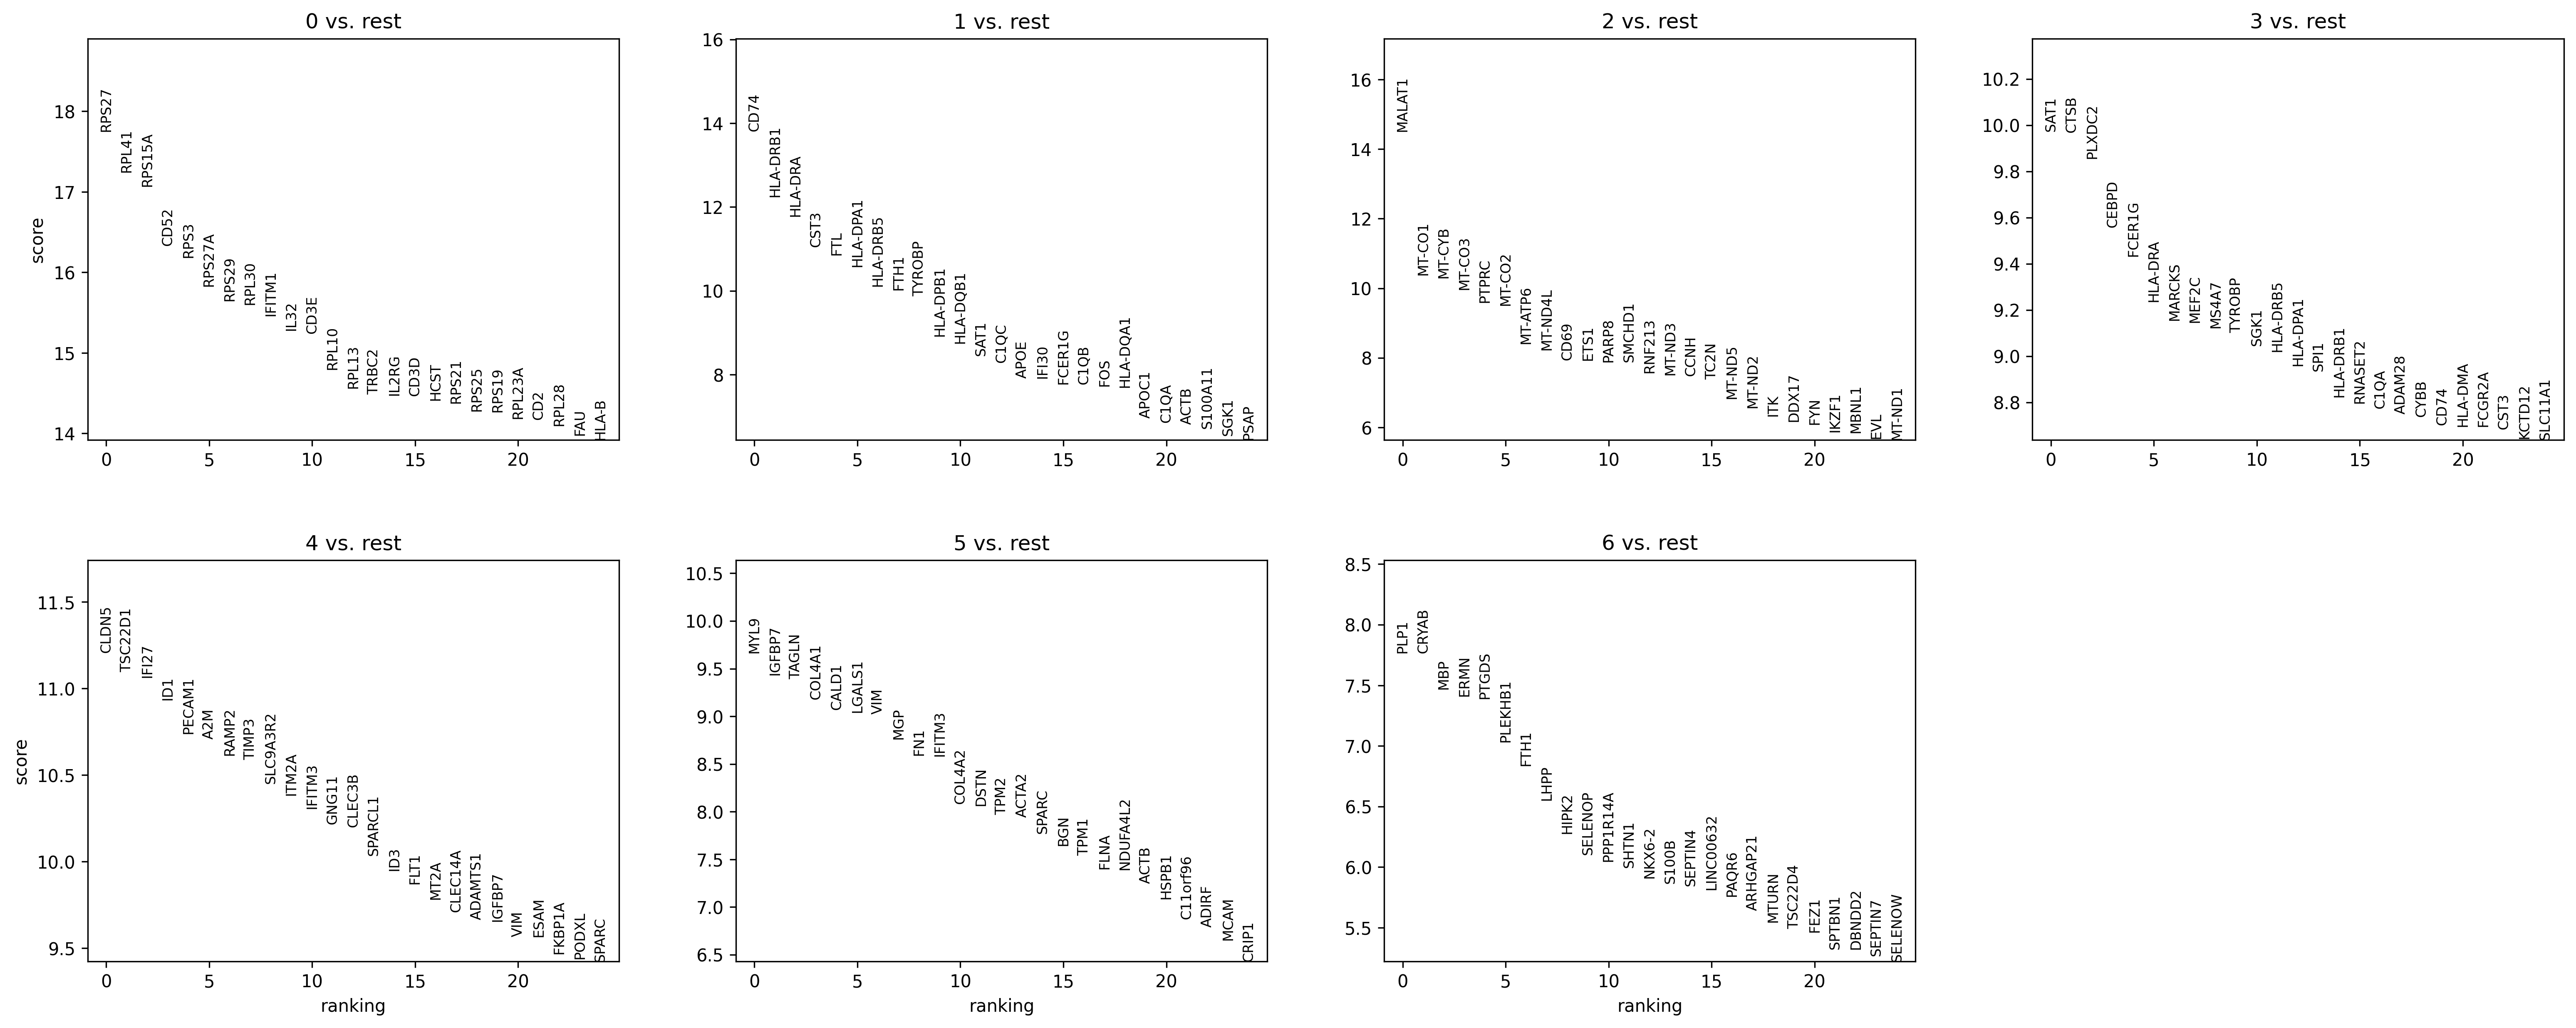
\includegraphics[width=0.8\textwidth]{de.png}
    \caption{Differential Expression Analysis}
    \label{fig:de}
\end{figure}

\end{document}
